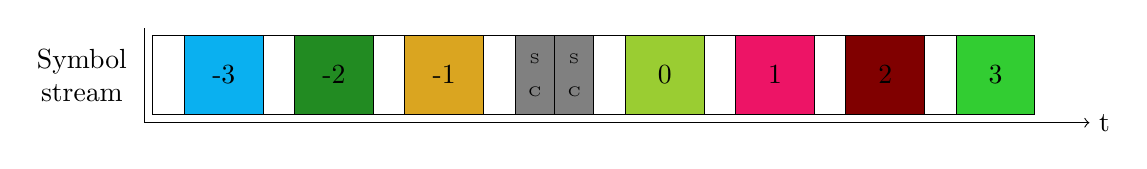
\begin{tikzpicture}
  \tikzset{
    sample/.style={minimum width=10mm, minimum height=10mm, anchor=south west, draw=black},
    rsc/.style={minimum width=5mm, minimum height=10mm, anchor=south west, draw=black, fill=white, align=center},
    rcp/.style={minimum width=4mm, minimum height=10mm, anchor=south west, draw=black, fill=white},
    rnarrow/.style={minimum width=1mm, minimum height=10mm, anchor=south west, draw=black, fill=white},
    wsample/.style={minimum width=13mm, minimum height=10mm, anchor=south west, draw=black},
    label/.style={anchor=east, align=center},
  }

  % time axis
  \draw[->]
  (0, 0) --
  (12, 0) node[anchor=west]{t};

  % other axis
  \draw
  (0, 0) --
  (0, 1.2);

  % Path 1
  \draw
  (0.1, 0.1) node[rcp]{}
  ++(0.4, 0) node[sample, fill=ProcessBlue]{-3}
  ++(1, 0)node[rcp]{}
  ++(0.4, 0) node[sample, fill=ForestGreen]{-2}
  ++(1, 0)node[rcp]{}
  ++(0.4, 0) node[sample, fill=Goldenrod]{-1}
  ++(1, 0)node[rcp]{}

  ++(0.4, 0) node[rsc, fill=Gray]{\tiny{S}\\\tiny{C}}
  ++(0.5, 0) node[rsc, fill=Gray]{\tiny{S}\\\tiny{C}}

  ++(0.5, 0)node[rcp]{}
  ++(0.4, 0) node[sample, fill=YellowGreen]{0}
  ++(1, 0)node[rcp]{}
  ++(0.4, 0) node[sample, fill=WildStrawberry]{1}
  ++(1, 0)node[rcp]{}
  ++(0.4, 0) node[sample, fill=Maroon]{2}
  ++(1, 0)node[rcp]{}
  ++(0.4, 0) node[sample, fill=LimeGreen]{3};

  \draw
  (-0.1, 0.6) node[label]{Symbol\\stream};
\end{tikzpicture}
